\chapter{Transmissão em redes sem fio}
\label{cap:transmissao-redes-sem-fio}

\section{O ESPECTRO ELETROMAGNÉTICO}
\label{sec:espectro-eletromagnetico}

Quando se movem, os elétrons criam ondas eletromagnéticas que podem se propagar pelo espaço livre (até mesmo no vácuo), transportando energia durante o percurso. Essas ondas foram previstas pelo físico inglês James Clerk Maxwell em 1865 e foram observadas pela primeira vez pelo físico alemão Heinrich Hertz em 1887 \cite{tanenbaum2011}. O número de ciclos (oscilações) por segundo de uma onda eletromagnética é chamado frequência, e é medido em Hertz (Hz) -- em homenagem a Heinrich Hertz. A distância entre dois pontos máximos (ou mínimos) consecutivos é chamada comprimento de onda, designada universalmente pela letra grega $\lambda$ (lambda).

A velocidade de uma onda qualquer depende do meio em que ela se propaga. No vácuo, todas as ondas eletromagnéticas viajam na mesma velocidade, a da luz, que é aproximadamente igual a $3 \times 10^8$ m/s, independentemente de sua frequência \cite{tanenbaum2011}.

Essas três grandezas -- frequência ($f$), comprimento de onda ($\lambda$) e velocidade ($c$) -- se relacionam (no vácuo) através da seguinte expressão:

\begin{equation}
	\begin{aligned}
		c = \lambda f
	\end{aligned}
\end{equation}

\begin{figure}[H]
	\centering
	\Caption{\label{fig:onda}Propriedades de uma onda.}	
	\UECEfig{}{
		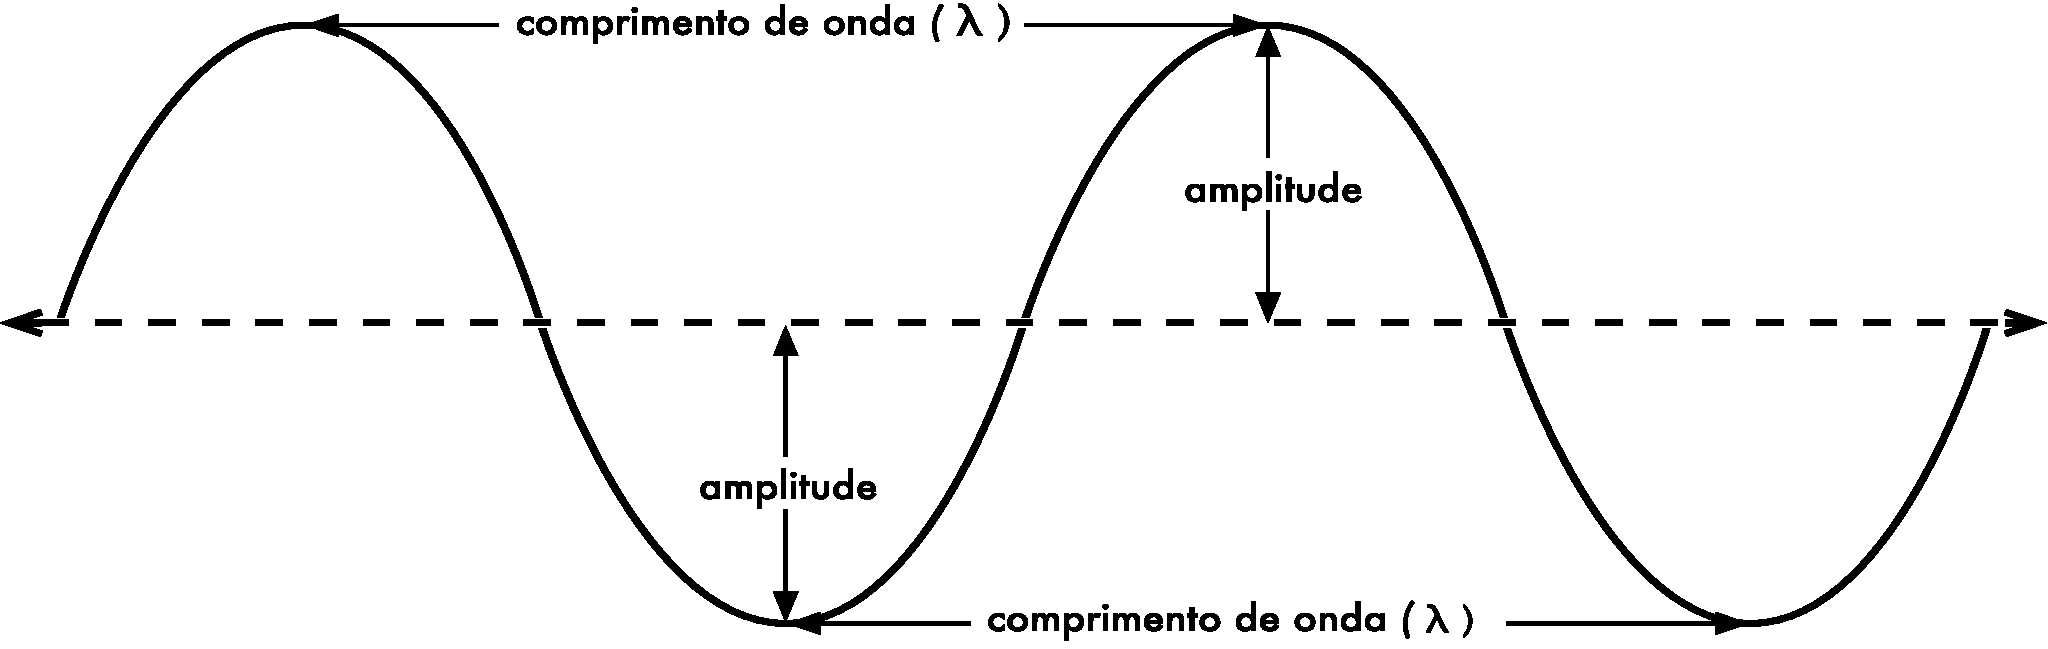
\includegraphics[scale=.4]{figuras/onda0.pdf}
	}{
		\Fonte{\citeonline[p. ~10]{flickenger2008}.}
	}	
\end{figure}

Uma vantagem da onda eletromagnética é o fato de que ela pode ser gerada ou captada por circuitos eletrônicos simples. Além disso, esse tipo de onda se propaga no vácuo, o que permite a comunicação entre antenas terrestres com satélites no espaço e vice-versa, entre os próprios satélites e entre dois pontos localizados em qualquer parte da superfície terrestre \cite{fluminense2010}.

Os dispositivos sem fio são restritos para operar em uma determinada banda (ou faixa) de frequência. Cada faixa tem uma largura de banda associada, que é simplesmente a quantidade de espaço de frequência na banda. Se a variação entre 2,40 GHz e 2,48 GHz é usada por um dispositivo, então a largura de banda será de 0,08 GHz ou 80 MHz.

A largura de banda adquiriu uma conotação de ser uma medida da capacidade de dados de um \textit{link}. Uma grande quantidade de matemática, teoria da informação e processamento de sinais pode ser usada para demonstrar que fatias mais largas de frequência podem ser usadas para transmitir mais informações \cite{gast2002}. Por exemplo, um canal de telefonia móvel analógico requer uma largura de banda de 20 kHz. Os sinais de televisão são muito mais complexos, já que, necessariamente, transmitem tráfego de áudio e vídeo, e por esse motivo possuem uma largura de banda consideravelmente maior, cerca de 6 MHz \cite{gast2002}.

O uso de uma faixa de frequência é rigorosamente controlado pelas autoridades reguladoras através de processos de licenciamento. No âmbito mundial, o processo de padronização de alocação de frequências para uso específico é realizado pela União Internacional de Telecomunicações (ITU, do inglês, \textit{International Telecommunication Union}). No Brasil, a ANATEL (Agência Nacional de Telecomunicações) representa a entidade responsável pela definição e fiscalização da utilização das faixas de frequência em território nacional. Essas determinações regulatórias visam coibir o uso das faixas de frequência sem permissão por infratores como estações de rádio e TVs piratas.

Entretanto, existem faixas de frequência que não estão sujeitas a autorização de uso pelos órgãos reguladores, ou seja, são bandas de frequência abertas para transmitir. Essas frequências não licenciadas são conhecidas como ISM (do inglês, \textit{Industrial, Scientific, Medical}). As bandas ISM foram padronizadas na maioria dos países em três faixas de frequência: 900 MHz, 2,4 GHz e 5 GHz \cite{moraes2010,tanenbaum2011}. A figura abaixo exibe a alocação das frequências ISM e também das bandas U-NII (do inglês, \textit{Unlicensed National Information Infrastructure}).

\begin{figure}[H]
	\centering
	\Caption{\label{fig:ism_unii}As bandas ISM e U-NII.}	
	\UECEfig{}{
		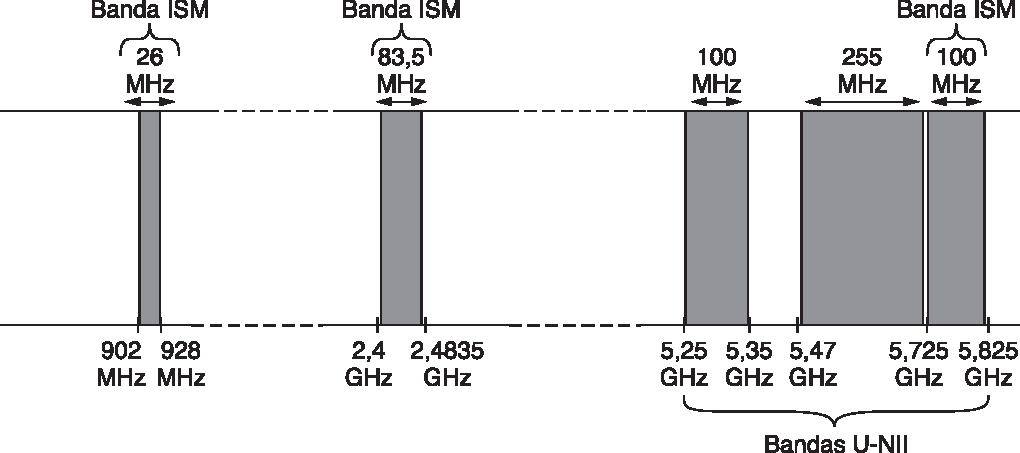
\includegraphics[scale=.6]{figuras/ism-unii.pdf}
	}{
		\Fonte{\citeonline[p. ~66]{tanenbaum2011}.}
	}	
\end{figure}

Cada banda de frequência utilizada nas telecomunicações estão contidas em um modelo de escala comum, onde é apresentado o intervalo completo de todas as possíveis frequências da radiação eletromagnética, denominado de espectro eletromagnético. A figura abaixo ilustra todas as variações de frequências contidas no espectro eletromagnético.

\begin{figure}[H]
	\centering
	\Caption{\label{fig:espectro}O espectro eletromagnético e a maneira como ele é usado na comunicação.}	
	\UECEfig{}{
		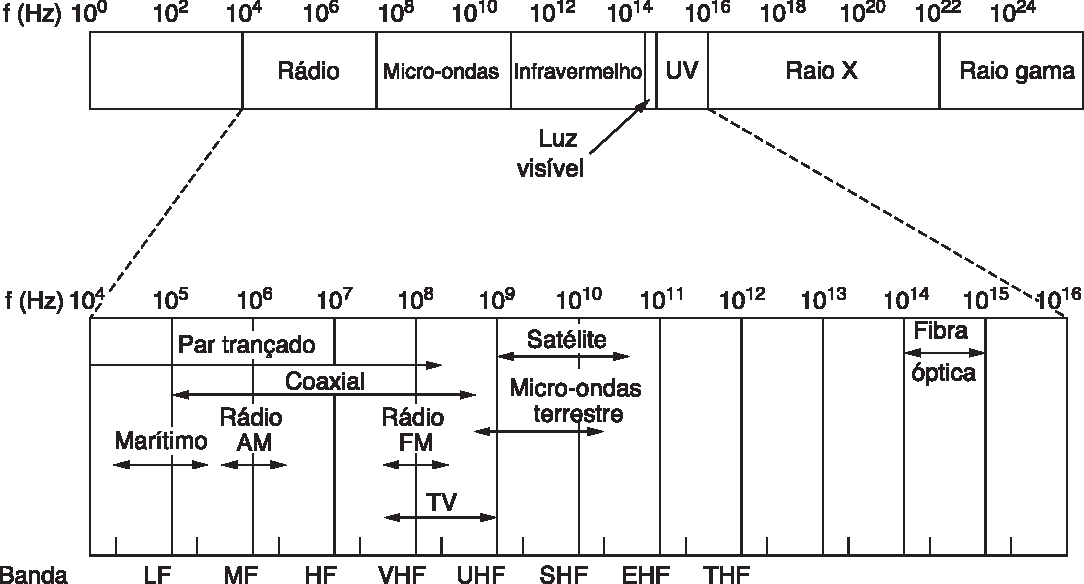
\includegraphics[scale=.72]{figuras/espectro_eletromagnetico.pdf}
	}{
		\Fonte{\citeonline[p. ~70]{tanenbaum2011}.}
	}	
\end{figure}

\begin{citacao}
	As faixas de rádio, microondas, infravermelho e luz visível do espectro podem ser usadas na transmissão de informações, por meio de modulação da amplitude, da frequência ou da fase das ondas. A luz ultravioleta, os raios X e os raios gama representariam opções ainda melhores, por terem frequências mais altas, mas são difíceis de produzir e modular, além de não se propagarem bem através dos prédios e de serem perigosos para os seres vivos \cite{tanenbaum2011}.
\end{citacao}